\documentclass[12pt]{article}
\usepackage{amsmath}
\usepackage{amssymb}
\usepackage{graphicx}
\usepackage[margin=1in]{geometry}
\newcommand{\del}{\nabla}
\begin{document}

\title{Psych209 Final Project}
\author{Howon Lee}
\maketitle

%explain the bak net
  How can you use extremal dynamics to train some kind of neural net?
  Qualitative model of evolution: Bak-Sneppen model.
  \begin{figure}
    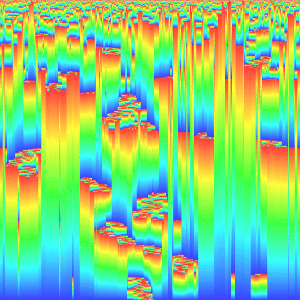
\includegraphics{bak_sneppen}
  \end{figure}

  Rules of Bak-Sneppen model. How does it behave? Criticality. Self-organized criticality.

  Caveats: CR Shalizi, W Tozier, "A Simple Model of the Evolution of Simple Models of Evolution"
  
  Bak and Chialvo's model

  More abstract: extremal optimization

  Finally: Using $\tau$-EO on RBM, classification results
  
  How it works, from 20000 feet
  \begin{figure}
    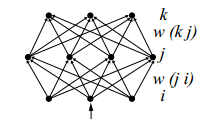
\includegraphics{bak_chialvo_net_topology}
  \end{figure}
  
  Problems: Conjunctive neurons
  \begin{figure}
    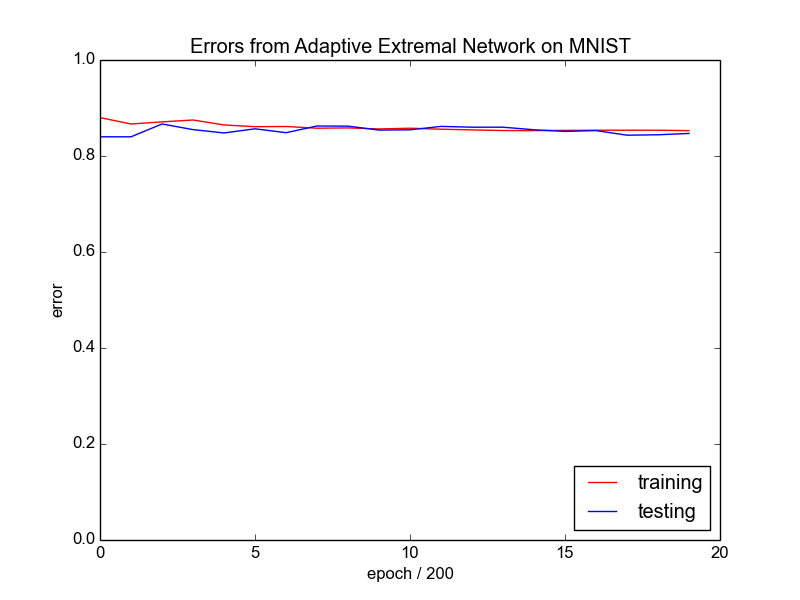
\includegraphics{bak_plot}
  \end{figure}

  Comparison to simulated annealing
  
  How it works, from 20000 feet

  Existing results, from Boetticher: TSP, Ising model

  $\tau$-EO
  
  \begin{figure}
    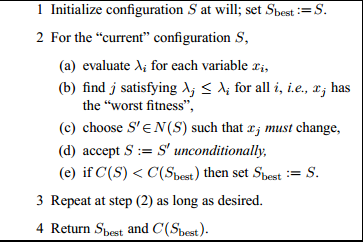
\includegraphics{eo_alg}
  \end{figure}
  
  The hope:
  \begin{figure}
    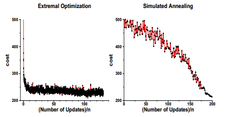
\includegraphics{boettcher}
  \end{figure}
  
  Why not feedforward? BM vs. Ising Model

  Locality: RBM

  \begin{figure}
    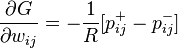
\includegraphics{rbm_eq}
  \end{figure}
  
  \frametitle{Ising Model}
  \begin{figure}
    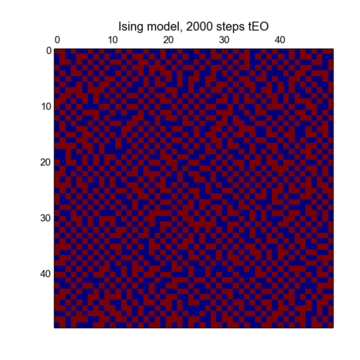
\includegraphics{2000}
  \end{figure}
  \begin{figure}
    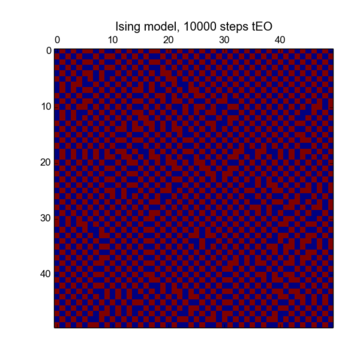
\includegraphics{10000}
  \end{figure}
  
  \frametitle{Ising Model}
  \begin{figure}
    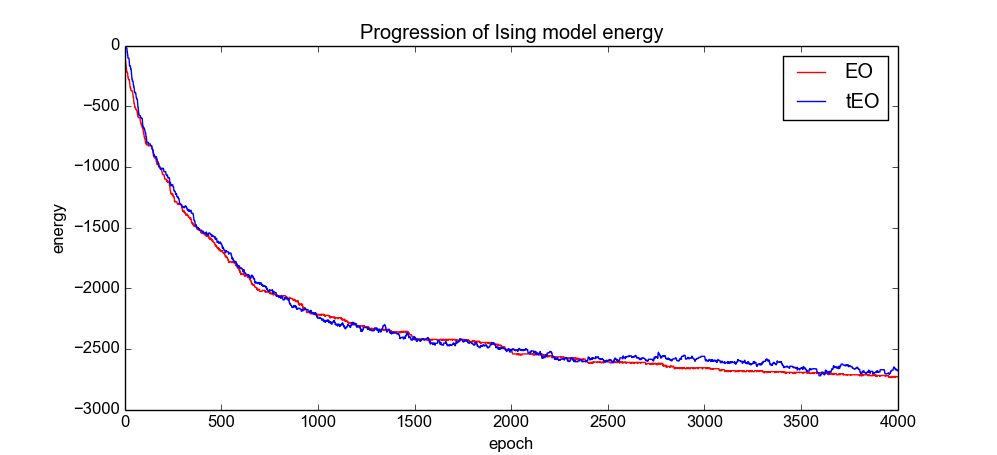
\includegraphics{ising_energy_unzoomed}
  \end{figure}
  
  \begin{figure}
    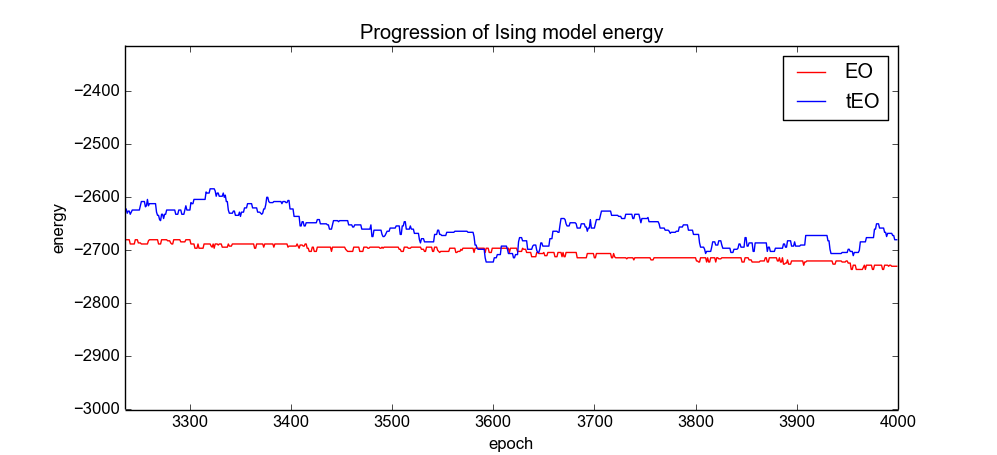
\includegraphics{ising_energy_zoomed}
  \end{figure}

  See performance in RBM learning, as simple as possible

  Bit string: metaphor of Hamming cliff in GA

  Actually, this is just a weird coordinate descent
  
  \begin{figure}
    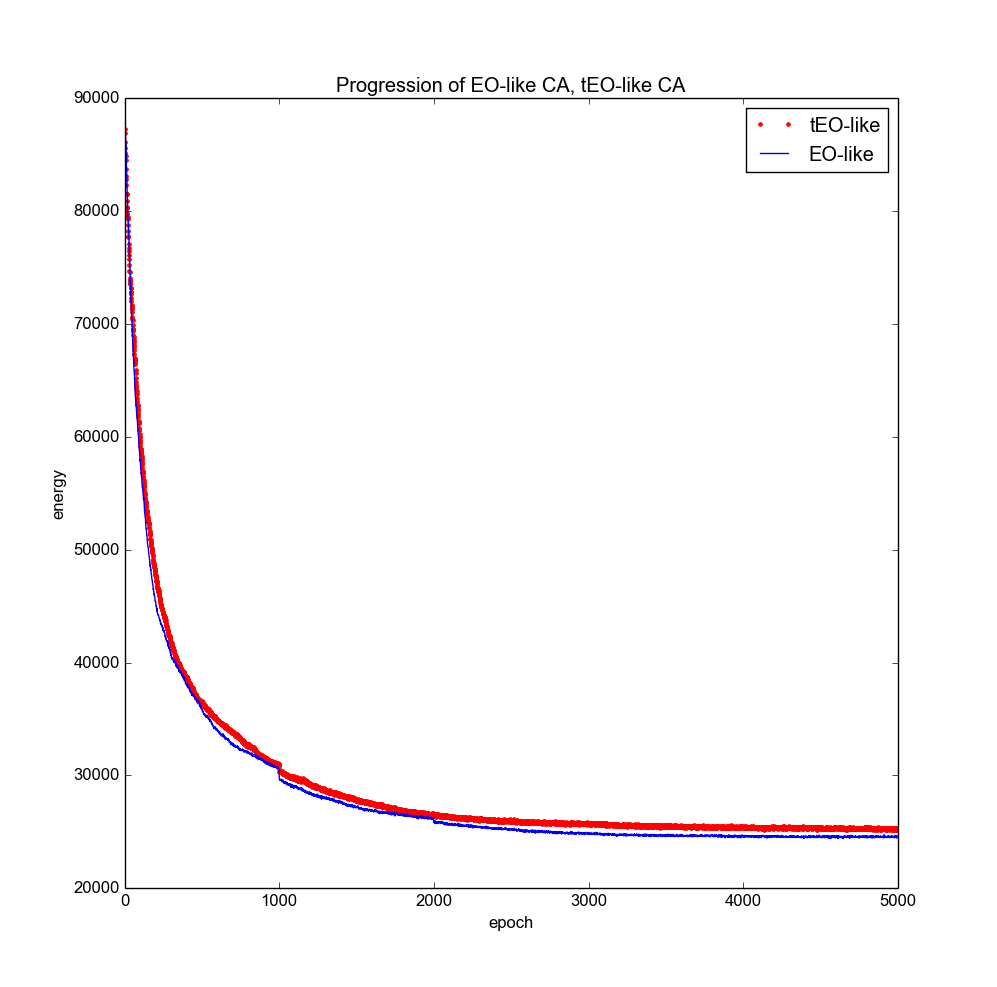
\includegraphics{eo_rbm_unzoomed}
  \end{figure}
 
  \begin{figure}
    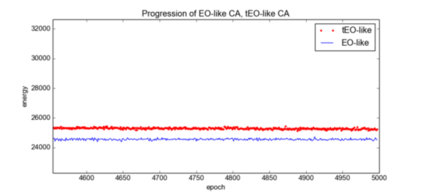
\includegraphics{eo_rbm_zoomed}
  \end{figure}

  Make an algorithm that actually differs from CDiv

  Try non-restricted RBM, and learn with regular gradient

  (using EO in place of SA)

%%%% organization

\section*{Issue Addressed} %What is the issue or question you will be addressing?

An alternative optimization algorithm called $\tau$-extremal optimization is used to update a constraint-satisfaction framework to escape local minima in short amounts of time. It is compared on a toy task (the Necker Cube task), but with every possible combination of initial input, and shown to do very well in comparison to a simulated-annealing Boltzmann machine with and without an annealing schedule.

\subsection*{Why is it interesting?}

The update rule for Boltzmann machines in the general, non-restricted case is very powerful but not usable in practice, because of the enormous time needed to approach the network's equilibrium distribution and the noisy learning signal for the learning.
%%%%%%%%%%%
\subsection*{What has previously been done?}
%%%%%%%%%%% tsp and spin glasses. really quite interesting in specific, because of the close relation between ising spin glasses and bm
\subsection*{What remains to be done?}
%%%%%%%%%%%

\section{Novel Approach}

I will try to use the method by Boetticher et al on the problem of taking equilibrium-like statistics from a Boltzmann machine, to see if it helps the current intractable problem of non-restricted Boltzmann machine learning. The method, called Extremal Optimization (EO), has been used in Ising model systems before (spin glasses modelled by an Ising model system), but not to the updating of a Boltzmann machine, to my knowledge. %%%% cite Boetticher and the Ising model tau-EO paper.

EO is a global optimization technique, inspired by a model of evolution proposed by Bak and Sneppen, and the qualitative results that result from that model. %%% bit of exegesis of Bak-Sneppen model; %%%% cite Bak-Sneppen paper

%% now finally explain EO
%% tau-EO

%%%In order to explain what EO is, it is helpful to have a prior picture of simulated annealing(SA). Both of these optimization techniques are attempts to solve the problem of local optima that all hill-climbing optimization algorithms are subject to. SA, in order to maximize a criterion, considers a neighboring state and takes or rejects the neighboring state based upon the Metropolis-Hastings criterion. That Metropolis-Hastings criterion depends upon a temperature which is varied during the course of the algorithm: this is called the annealing schedule. A high temperature allows more thorough exploration of the solution space and a low temperature allows more bias towards an optimum solution. Together, they are a global optimization algorithm.
%% compare and contrast EO, SA

%What approach will you be taking to address it? (at a big picture level; novel and/or otherwise noteworthy aspects)

\section{Details of Approach}

%Specific target phenomenon or phenomena you will be addressing: e.g., pattern of data you intend to try to fit. Model network task setting, architecture, processing and learning algorithm, training environment (corpus used for training, knowledge base built in to network),

%%% note the bak net try
%%% note the rbm try
%%% going to note the fact that I did bm normally now

\section{Results and Analysis}

%%First present your primary findings that bear directly on the target phenomena.
%%% it's faster

%%A strong paper will, in addition, present an analysis of why the results came out the way they did, especially in cases where results did not come out as expected. 
%%% why is it faster?
%%% note the fasterness of SA compared to schedule SA is partly an artifact of the fact that we demand a global minima: the schedule tends to get stuck in local minima
%%% but why is the tauEO faster? immediately after it makes a huge jump to escape local minima, the power law distribution of tau means that it will tend to explore the new local state space really fast, for basically the same reason that it's an online algorithm.

%%It can be useful to discuss results you obtain with one of us to get suggestions as to how to fully understand your findings.

%%Analysis not only of network outputs but also of the structure of the information present in the materials you use to train your network (when relevant) and / or the hidden unit activations, network weights, or learning trajectory can help illuminate why and how your network has performed the way it did.

\section{Discussion}

%%% theoretical thoughts: online algorithm
%%% theoretincal thoughts: out of equilibrium
%%% theoretical thoughts: black magic in determining the number of iterations, very associated with the fact of being an online algorithm

%Summarize your goals, your approach, and your main findings, and state a conclusion indicating how well, overall, your goals have been met.

%%% goals: make a faster thing than SA for abstract csp
%%% approach: tau-EO for cs net
%%% findings: spiffy results
%Then, discuss shortcomings or limitations of your effort and indicate how these might be overcome in future work.
%%% limitations: limited net, not fully connected, not a real problem. doesn't scale up.
%%% limitations: not thinking hard about neuronal connectivity. one thing that continues on the subject of criticality is modelling chialvo's work
%%% broader implications: try to look carefully at the critical regions of abstract NP-complete problem
%%Also, indicate broader implications and potential future applications of the ideas and approach.

\section{Summary}

Citations:   We will not be sticklers for details of citation styles but do provide citations to literature you draw on in your paper, using the following format

\end{document}

